\section{Parser Combinators for Path Querying}
\label{sec:combinators}

Parser combinators is a way to specify both a language syntax and a parser for it in terms of higher-order functions.
Parser in this framework is a function which consumes a prefix of an input and returns either a parsing result or an error if the input is erroneous.
Parser combinators compose parsers to form more complex parsers.
A parser combinators library usually provides a set of basic parser combinators, such as a combinator of the sequential application or of the choice, but there can also be user-defined combinators.
Most parser combinators libraries, including the Meerkat library, can only process the linear input---strings or some kind of streams.
We modify the Meerkat library to work on the graph input. The following ideas are at the core of the modification.

The intersection of a context-free and a regular language is context-free. There are several constructive proofs of this fact.
The proposed solution is yet another constructive proof with the SPPF as a user-friendly representation of the context-free grammar for the intersection.

Linear input can be regarded as a linear directed graph with symbols of the input labeling the edges.
A conventional parser moves a pointer in the input from the position $i$ to the position $i+1$ and creates a new state when a token between the $i$-th and the $i+1$-th positions matches what is required in the grammar.
In case of graph processing, there are possibly multiple ways to move from the current vertex $i$ and it is possible to produce multiple new states.
Generalized parsing is designed to optimally handle the production of multiple new states thus it is suitable to handle graph processing.

Matching a token in the input can be viewed as a predicate, for example $p_c (x) = x == c$.
We can generalize this observation allowing matching of an edge label of an arbitrary type with a predicate of some sort.
If vertices of the graph contain any data of interest, we can treat them in the similar fashion as the edges.
The formal definition of the context-free language constrained path querying changes only in a way a string is collected along a path in the input graph: the data stored in the vertices should also be taken into consideration.

Handling cycles in the input graphs imposes two challenges: not to get stuck in an infinite loop while processing the positions and if a new parsing state appears at some position, all paths which pass through this state, should be accounted for.
Both of these challenges are solved by the Meerkat memoization routine.
Parsing from a parser state at each position is only run if it has never been run before, so since there is only a finite number of parsing states and positions in the input, parsing terminates.
Appearing of the new parsing state at a position which has been processed before triggers processing of every path possibly affected by it.
Thanks to the memoization, each derivation of each subpath is analyzed only once, so there are no significant overhead at re-running.


Querying process in our library is inherited from generalized parsing and is done in two steps.
The first step is ``parsing'': the construction of the SPPF which contains all derivation trees for the paths satisfying syntactic constraints.
The second step is semantic actions application which retrieves the necessary additional data about the paths from the SPPF.

\subsection{The Set of Combinators}

We demonstrate the set of combinators by example: the input graph, which represents a map, is presented in Fig.~\ref{fig:graph}.
There are some cities connected by one-way roads represented by the edges labeled $road\_to$.
Each city is labeled by its name and a country it belongs to.

\begin{figure}[h]
\resizebox {0.45\textwidth} {!}
{
\begin{tikzpicture}[shorten >=1pt,node distance=2cm,on grid,auto]
   \node[state] (a) [fill={rgb:black,1;white,2}]  {$a(X)$};
   \node[state] (b) [right=of a] {$b (Y)$};
   \node[state] (c) [right=of b] {$c (X)$};
   \node[state] (d) [left=of a] {$d (Y)$};
   \node[state] (e) [left=of d] {$e (X)$};
    \path[->]
    (a) edge [bend left, above] node [above] {$road\_to$} (c)
    (b) edge  node {$road\_to$} (a)
    (c) edge  node {$road\_to$} (b)
    (a) edge  node {$road\_to$} (d)
    (d) edge  node {$road\_to$} (e);
\end{tikzpicture}
}
\caption{Example graph. Vertex labels are in the form "city-name (country-name)"}
\label{fig:graph}
\end{figure}

Two basic building blocks of queries are the combinators for dealing with edges and vertices.
\begin{itemize}
    \item \lstinline{V[N](predicate: N =>   Boolean)} the combinator for processing vertices, where \lstinline{N} is a type of the node label.
    Parsing with this combinator succeeds iff the vertex satisfies the predicate.
    \item \lstinline{E[L](predicate: L =>   Boolean)} the combinator for processing edges, where \lstinline{L} is a type of the edge label.
    Parsing with this combinator succeeds iff the edge satisfies the predicate.
\end{itemize}

\begin{figure}[h]
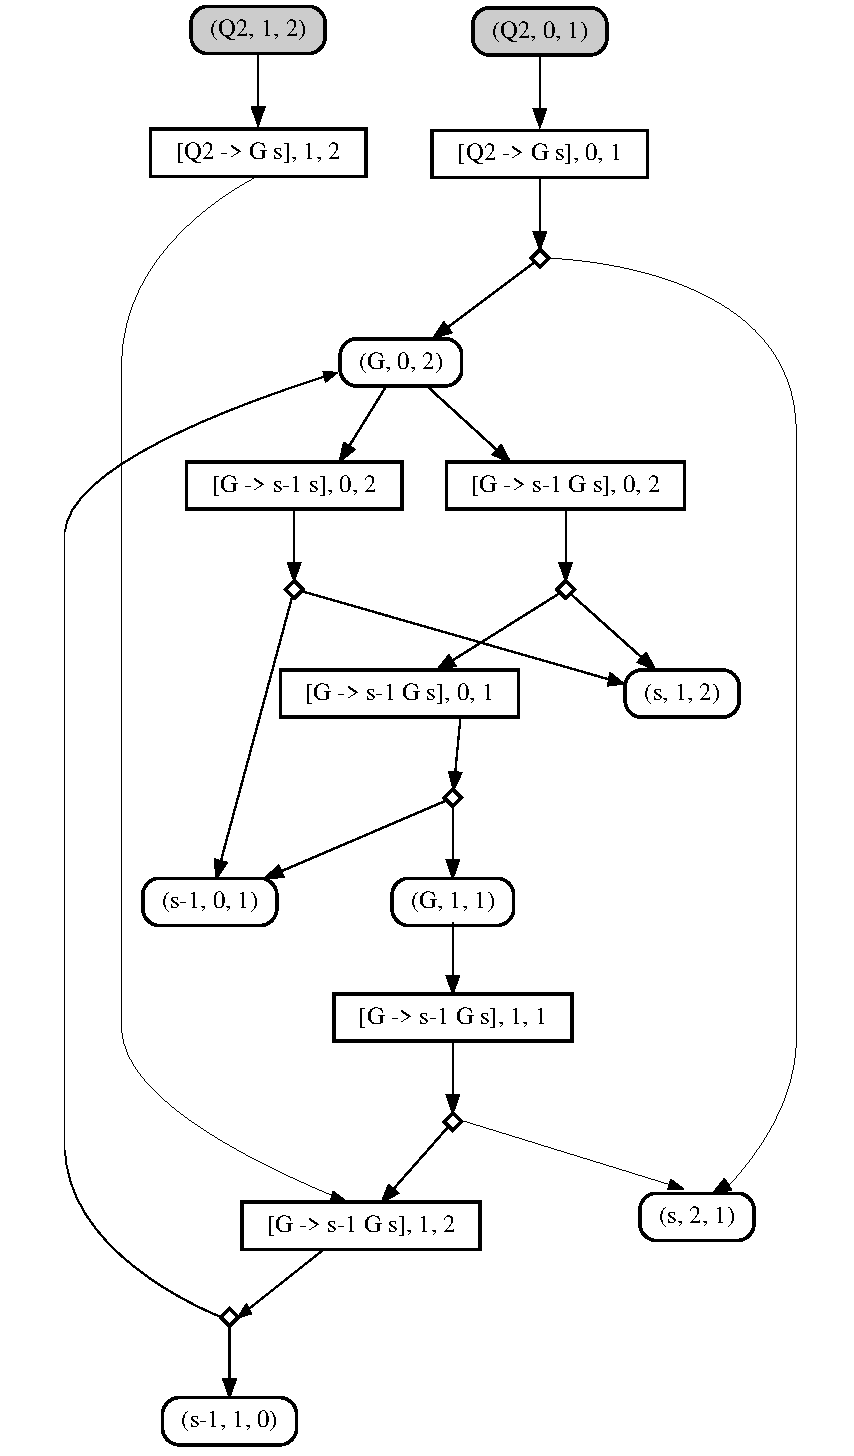
\includegraphics[width=0.49\textwidth]{sppf}
\caption{SPPF: result of applying cities query to the graph~\ref{fig:graph}}
\label{fig:sppf}
\end{figure}

To select cities which belong to some country, we can use the function \lstinline{V}: \lstinline{V[N]((e: Entity) =>   e.country =   "County Name")}.
Here \lstinline{Entity} is a property container for both edges and vertices.
By using the \lstinline{Dynamic} trait, all accesses to properties (like \lstinline{(e: Entity).country}) are converted to the accesses to the properties of either a vertex or an edge.
For the sake of simplicity, we will omit \lstinline{Entity} type specifications for predicates.
To query the graph for the paths from a city in the country $X$ to a city in the country $Y$, we need to sequentially compose the combinators for selecting the appropriate cities.
A sequentialital combinator \lstinline{~} does just that: it sequentially  applies two queries one after the other.
Let us denote a query for retrieving a city from the specific country \lstinline{city(name: String)} and a query for retrieving road edges \lstinline{roadTo}.
With this denotation, a query \lstinline{city("X") ~ roadTo ~ city("Y")} returns the requested set of paths from the graph.
The complete query with all necessary subqueries is shown in Fig.~\ref{fig:simpleQuery}.

\begin{figure}[h]
\begin{lstlisting}
def city(country: String) = V(_.country == country)
val roadTo = E(_.value() == "road_to")
val ourPath = city("X") ~ roadTo ~ city("Y")
\end{lstlisting}
\caption{Path query}
\label{fig:simpleQuery}
\end{figure}

Having the query written, the next thing is to write a function to retrieve the actual data about the paths.
If we care only about the names of the cities, we can return a pair of the cities for each path.
First, we modify the query for vertices by adding the semantic action to it using the combinator \lstinline{^}: \lstinline{def city(name: String) =    syn(V(e.value() ==   name) ^ (_.value))}\footnote{Underscore in anonymous lambda functions serves as a placeholder for an argument: \lstinline{(_.f)} is equavalent to \lstinline{(x => x.f)} }.
Then we need to actually map a path to a pair of cities: this is done with the combinator \lstinline{&}.
The complete query is in Fig.~\ref{fig:simpleQueryV2}.
The result is the sequence of pairs of cities with the road between them.

\begin{figure}[h]
\begin{lstlisting}
def city(country: String) =
  syn(V(_.country() == country) ^ (_.name))
val roadTo = E(_.value() == "road_to")
val ourPath =
  syn(city("X") ~ roadTo ~ city("Y") &
    { case c0 ~ c1 => (c0, c1 })
\end{lstlisting}
\caption{Path query}
\label{fig:simpleQueryV2}
\end{figure}


The whole set of basic combinators, which our library provides, is presented in Table~\ref{table:combinators}.
There are two kinds of combinators: the first kind combines parsers to form new parsers, meanwhile the second one is dedicated to the processing of the query result.
Whenever a string is used within a query, a parser which matches that string is implicitly generated.

\begin{table}[h]
\centering
\begin{tabular}{l@{}|l}
\multicolumn{1}{c|}{Combinator} & \multicolumn{1}{|c}{Description} \\ \hline
{\lstinline!a ~ b!} & sequential parsing: {\lstinline!a!} then {\lstinline!b!}   \\
{\lstinline!a | b!} & choice: {\lstinline!a!} or {\lstinline!b!}         \\
{\lstinline!a ?!}   & optional parsing: {\lstinline!a!} or nothing   \\
{\lstinline!a *!}   & repetition of zero or more {\lstinline!a!} \\
{\lstinline!a +!}   & repetition of at least one {\lstinline!a!} \\
{\lstinline!a ^ f!} & apply {\lstinline!f!} function to {\lstinline!a!} if  {\lstinline!a!} is a token \\
{\lstinline!a ^^!}  & capture output of {\lstinline!a!} if {\lstinline!a!} is a token    \\
{\lstinline!a & f!} & apply {\lstinline!f!} function to {\lstinline!a!} if  {\lstinline!a!} is a parser \\
{\lstinline!a &&!}  & capture output of {\lstinline!a!} if {\lstinline!a!} is a parser    \\
\hline
\end{tabular}
\caption{Meerkat combinators}
\label{table:combinators}
\end{table}


\subsection{Generic Interface for Input}
The combinators in our library are independent of the input representation.
It is enough to specify two basic combinators which handle vertices and edges.
Vertex handling is checking whether the vertex satisfies the given predicate.
In case of the edges, one needs to check which of the edges outgoing from the given vertex satisfy the given predicate.
These two functions form the trait for the input (Fig.~\ref{fig:input}).
It has two type parameters: the type of edge labels \lstinline{L} and the type of vertices labels \lstinline{N}.
Since the required functions are simple, we believe it is possible to support most storages of graph-structured data.
We supported several different input sources:

\begin{itemize}
    \item Neo4jInput --- input source for the graph database Neo4j;
    \item GraphxInput --- input source for the graph presented in memory using GraphX library;
    \item LinearInput --- input source for the linear input data such as the ordinary strings.
\end{itemize}

\begin{figure}[h]
\begin{lstlisting}
trait Input[+L, +N] {
  def filterEdges(nodeId: Int,
      predicate: L => Boolean): Seq[(L, Int)]
  def checkNode(nodeId: Int,
      predicate: N => Boolean): Option[N]
}

\end{lstlisting}
\caption{Generalized input interface}
\label{fig:input}
\end{figure}

\subsection{Semantic Actions}
\label{sec:semanticActions}

Every path, which the query produces, has a derivation tree stored in the SPPF.
The derivation tree is a very rich structure which can be hard to understand.
To retrieve the data actually useful for the user, the library provides a mechanism of semantic actions.
It is a way to apply some function to a parsed token or a subsequence.

Semantic action binder for the tokens---vertices and edges alike---is \lstinline{^}. The most common use for it is to extract properties from the token and combine them in some fashion.

\begin{lstlisting}
// Defined in Terminal[+L] (edge) parser
def ^[U](f: L => U) =
  new SymbolWithAction[L, Nothing, U] {...

// Defined in Vertex[+N] parser
def ^[U](f: N => U) =
  new SymbolWithAction[Nothing, N, U] {...
\end{lstlisting}

For the combination of parsers there is a \lstinline{&} binder. Being  applied to a sequence of tokens, it can collect and process the data returned by the terminal parsers.
\begin{lstlisting}
// Defined in Symbol[+L, +N, +V] parser
def &[U](f: V => U) =
  new SymbolWithAction[L, N, U] {...
\end{lstlisting}

They both produce a new parser that parses the input exactly like the given parser but also have a bound function.
The function is referenced in each SPPF node produced by the corresponding parser.

The way semantic actions are executed has mostly remained the same as in the original Meerkat library: semantic actions are first executed for the children of the current node, then the results are collected and passed to a semantic action of the current node.
If there are ambiguous nodes in the SPPF, the original Meerkat library just throws an exception.
In our case, ambiguity can arise not only when there are multiple derivations of a string but ambiguous nodes can also represent several different subpaths which are derived from the respective nonterminal.
We chose to provide a way to extract the derivation trees from the SPPF lazily, since the number of the paths can be infinite.
Unambiguous trees are yielded with a breadth-first search.

The composition of the extraction of trees and the semantic action execution is called \lstinline{executeQuery}.
It parses the input graph from all positions, produces a list of SPPF roots, extracts all derivations from every root, executes semantic actions and returns a lazy stream of results.